\documentclass[a4]{article}

% PAQUETES %%%%%%%%%%%%%%%%%%%%%%%%%%%%%%%%%%%%%%%%%%%%%%%%%%%%%%%%%%%%%%%%%%%%%
\usepackage[utf8]{inputenc}
\usepackage{xcolor}
\usepackage{hyperref}
\usepackage{listings}
\usepackage{framed} % Para crear cuadros alrededor del texto

\usepackage[english]{babel}
%
\usepackage[fixlanguage]{babelbib}
    \bibliographystyle{IEEEtran}

\usepackage{url}

%!TEX encoding = UTF-8 Unicode
% !TEX spellcheck = es

\setlength{\textwidth}{6.5 in}
\setlength{\textheight}{8.5 in}
\setlength{\headsep}{0.3 in}

\usepackage{multirow, array} % para las tablas
\usepackage{float} % para usar [H]
\usepackage{charter}

% \usepackage[breaklinks=true]{hyperref}

%
% ADD PACKAGES here:
%

\usepackage{minted}


\usepackage[utf8]{inputenc}
\usepackage{amsmath,longtable,siunitx, float, graphicx, dcolumn, bm, fancyhdr, authblk, subcaption, caption, hyperref, multicol, setspace}

\usepackage{bbding}
\usepackage{amssymb}
\usepackage[rightcaption]{sidecap}
%\usepackage{textcomp}

\usepackage[hmarginratio=1:1, top=32mm, columnsep=20pt, headsep=\dimexpr20mm, margin=0.8in, top=1.3in ]{geometry}

\usepackage{booktabs}
\usepackage{multirow}

\usepackage{algorithm}
\usepackage{enumitem}
\usepackage{tabularx}
\usepackage[noend]{algpseudocode}
\usepackage{xcolor}

\newcommand{\TODO}{\textbf{\textcolor{red}{TODO}}}

\renewcommand{\algorithmicrequire}{\textbf{Input:}}
\renewcommand{\algorithmicensure}{\textbf{Output:}}

\newtheorem{theo}{Theorem}
\newenvironment{theorem}
  {\begin{mdframed}\begin{theo}}
  {\end{theo}\end{mdframed}}
  
\newtheorem{prop}{Proposición}
\newenvironment{proposition}
  {\begin{mdframed}\begin{prop}}
  {\end{prop}\end{mdframed}}

\newtheorem{lem}{Lema}
\newenvironment{lema}
  {\begin{mdframed}\begin{lem}}
  {\end{lem}\end{mdframed}}
  
\newtheorem{defi}{Definition}
\newenvironment{definition}
  {\begin{mdframed}\begin{def}}
  {\end{def}\end{mdframed}}
  
 \newtheorem{dm}{Demostración}

\usepackage[numbers]{natbib}
\usepackage{tocloft} % Añadir para ajustar la tabla de contenidos

% Configurar numeración arábiga en secciones
\renewcommand{\thesection}{\arabic{section}}

% Configurar interlineado simple en la tabla de contenidos
\setlength{\cftbeforesecskip}{0.8em}

\setlength{\parskip}{8pt}

% Definir el estilo de página
\pagestyle{fancy}
\fancyhf{} % Borrar todos los estilos de encabezado y pie de página
\fancyhead[L]{ % Encabezado izquierdo
    \begin{picture}(0,0)
        \put(0,-40){
\includegraphics[width=3cm]{img/uniandes_logo.png}} % Cambia "ejemplo.png" por el nombre de tu imagen y ajusta el ancho
    \end{picture}
}
\fancyfoot[R]{\thepage}
\renewcommand{\headrulewidth}{0pt} % Ajustar el grosor de la línea horizontal en el encabezado


\begin{document}
\singlespacing

\begin{titlepage}

\newcommand{\HRule}{\rule{\linewidth}{0.5mm}} % Defines a new command for the horizontal lines, change thickness here

\center % Center everything on the page
 
%----------------------------------------------------------------------------------------
%	HEADING SECTIONS
%----------------------------------------------------------------------------------------

\textsc{\LARGE Universidad de los Andes}\\[1.5cm]

\includegraphics[scale=.15]{img/uniandes_logo_2.png}\\[1cm]
\textsc{\Large Natural Language Processing}\\[0.5cm]
\textsc{\Large ISIS 4221}\\[0.5cm]


\HRule \\[0.4cm]
{ \huge \bfseries Tarea 4}\\[0.4cm] 
\HRule \\[3cm]

%-------------------------------------
%	AUTHOR SECTION
%-------------------------------------

\begin{center} \large
\emph{Autores:}\\
Isabella \textsc{Martínez}\\
Gustavo \textsc{Mendez}\\
Paula \textsc{Daza}\\
Nicolás \textsc{Klopstock}\\
\end{center}

\vfill % Move the date down the page
{\large Octubre 10, 2024}\\[2cm]

\end{titlepage}


\renewcommand{\contentsname}{Tabla de contenidos}
\tableofcontents
\newpage

\section{Introducción}

Esta tarea se centra en el uso de técnicas vistas en clase para entrenar modelos de representación de palabras y construir clasificadores basados en redes neuronales. El primer enfoque consiste en la selección de libros de tres autores del Proyecto Gutenberg, utilizando sus obras literarias para entrenar embeddings de palabras mediante la librería GENSIM y el modelo Word2Vec. Estos embeddings se deben graficar en una dimensionalidad reducida para explorar relaciones semánticas a través de las representaciones. Posteriormente, se desarrollarán modelos de clasificación multinomial para predecir el autor de fragmentos de texto, utilizando tanto embeddings entrenados como pre-entrenados de fuentes como Google-Word2Vec o Glove, para finalmente comparar los resultados obtenidos en términos de precisión, exactitud y recall.

\section{Preprocesamiento de Datos}
Para la carga y preprocesamiento de los textos, se utiliza el corpus de Project Gutenberg, que contiene libros de autores como Jane Austen, Arthur Conan Doyle y Edgar Allan Poe. El preprocesamiento incluye:
\begin{itemize}
    \item Normalización del texto: conversión a minúsculas y eliminación de puntuación.
    \item Eliminación de \textit{stopwords} utilizando la librería \texttt{nltk}.
    \item Lemmatización para reducir las palabras a su forma base.
    \item Segmentación del texto en fragmentos de 250 palabras, con una superposición de 200 palabras entre fragmentos consecutivos.
\end{itemize}

\section{Análisis de Datos}

\subsection{Creación del Modelo Word2Vec}

Para este análisis, aplicamos Word2Vec a un corpus seleccionado compuesto por obras de tres autores reconocidos: Jane Austen, Edgar Allan Poe y Arthur Conan Doyle. Los libros fueron obtenidos de Project Gutenberg, seleccionando las tres obras más descargadas de cada autor. El texto preprocesado se tokenizó, eliminando puntuación, y las palabras fueron lematizadas a sus formas base. También se eliminaron las \textit{stopwords} utilizando la librería NLTK, asegurando que solo se retuviera el contenido significativo para el entrenamiento del modelo.

Los pasos clave para la creación de los modelos Word2Vec fueron los siguientes:
\begin{itemize}
    \item \textbf{Preprocesamiento del texto}: El texto original se convirtió a minúsculas, se eliminó la puntuación y se excluyeron las \textit{stopwords}. La lematización permitió que diferentes formas de una palabra (por ejemplo, "caminando" y "caminó") se trataran como la misma palabra.
    \item \textbf{Entrenamiento de Word2Vec}: Entrenamos modelos Word2Vec con tres tamaños de embeddings: 100, 200 y 300. Cada modelo fue entrenado utilizando la arquitectura \textit{skip-gram}, que es efectiva para capturar relaciones semánticas entre palabras en un contexto determinado.
\end{itemize}

El proceso de entrenamiento consistió en iterar sobre los textos preprocesados y generar embeddings que capturaran las relaciones semánticas entre palabras. Los modelos Word2Vec se guardaron para un posterior análisis y visualización.

\subsection{Visualización de Embeddings}

Para explorar las relaciones semánticas codificadas por los embeddings entrenados, visualizamos las palabras y sus vecinos más cercanos utilizando el algoritmo t-SNE para la reducción de dimensionalidad. Este método nos permitió graficar los embeddings de alta dimensionalidad en un espacio bidimensional, proporcionando una representación clara de cómo las palabras se agrupan en función de sus similitudes contextuales. El algoritmo t-SNE se centra en mantener las relaciones \textit{locales} entre las palabras, es decir, mantiene las proximidades entre aquellas que comparten contextos similares en el espacio original de alta dimensionalidad. Esto se logra mediante la conversión de las distancias en probabilidades de vecindad tanto en el espacio original como en el espacio reducido, garantizando que los puntos cercanos permanezcan juntos luego de la transformación. Entonces, t-SNE facilita la identificación visual de grupos semánticamente relacionados, revelando patrones y estructuras latentes que de otro modo serían difíciles de observar.

Para cada autor, seleccionamos personajes o conceptos clave y visualizamos las palabras más similares a estos. Por ejemplo:
\begin{itemize}
    \item En \textbf{Emma} de Jane Austen, visualizamos las relaciones en torno a la palabra "Emma", mostrando fuertes conexiones contextuales con términos como "Mr", "Knightley" y "Harriet".

    \begin{figure}[H]
        \centering
        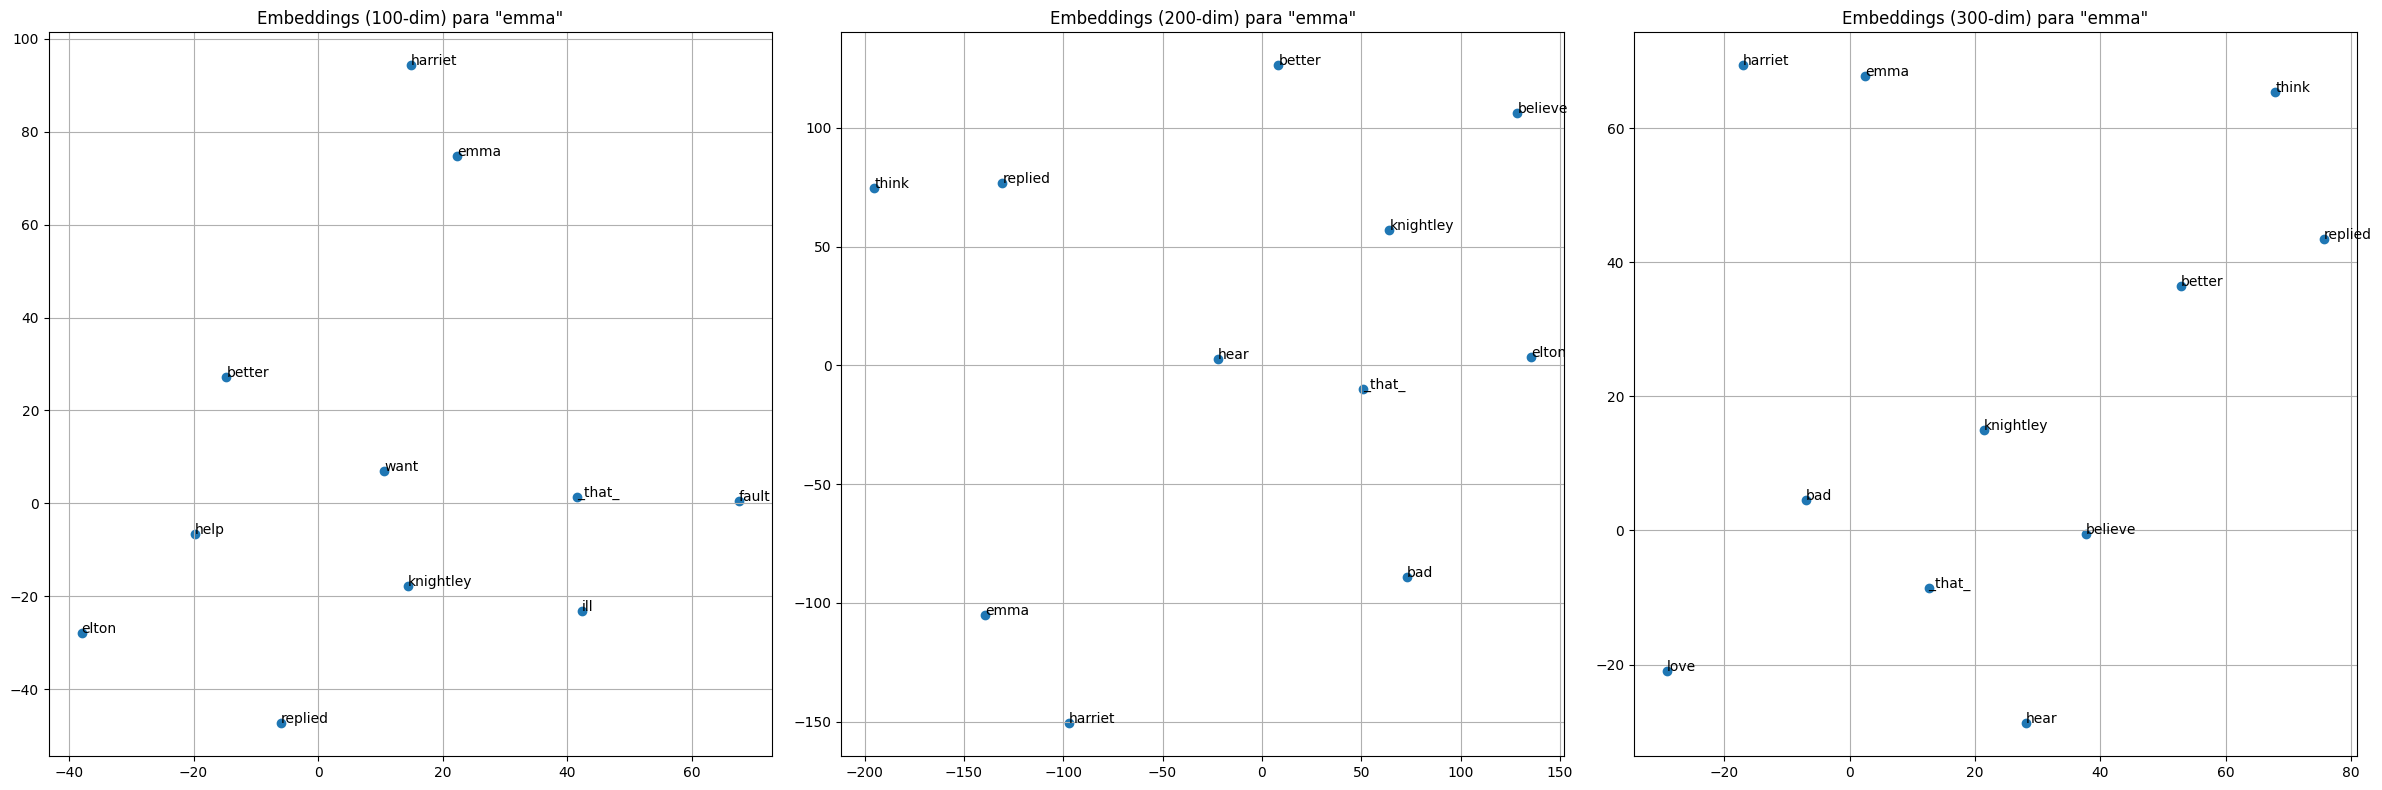
\includegraphics[width=0.9\textwidth]{img/emma_embeddings.png}
        \caption{Representación 2D de embeddings para "Emma" de "Emma" (100-dim, 200-dim \& 300-dim).}
        \label{fig:emma_embeddings}
    \end{figure}
    
    \item En \textbf{Orgullo y Prejuicio}, nos centramos en "Elizabeth", mostrando su relación semántica con palabras como "Darcy", "hermana" y "Bennet".

    \begin{figure}[H]
        \centering
        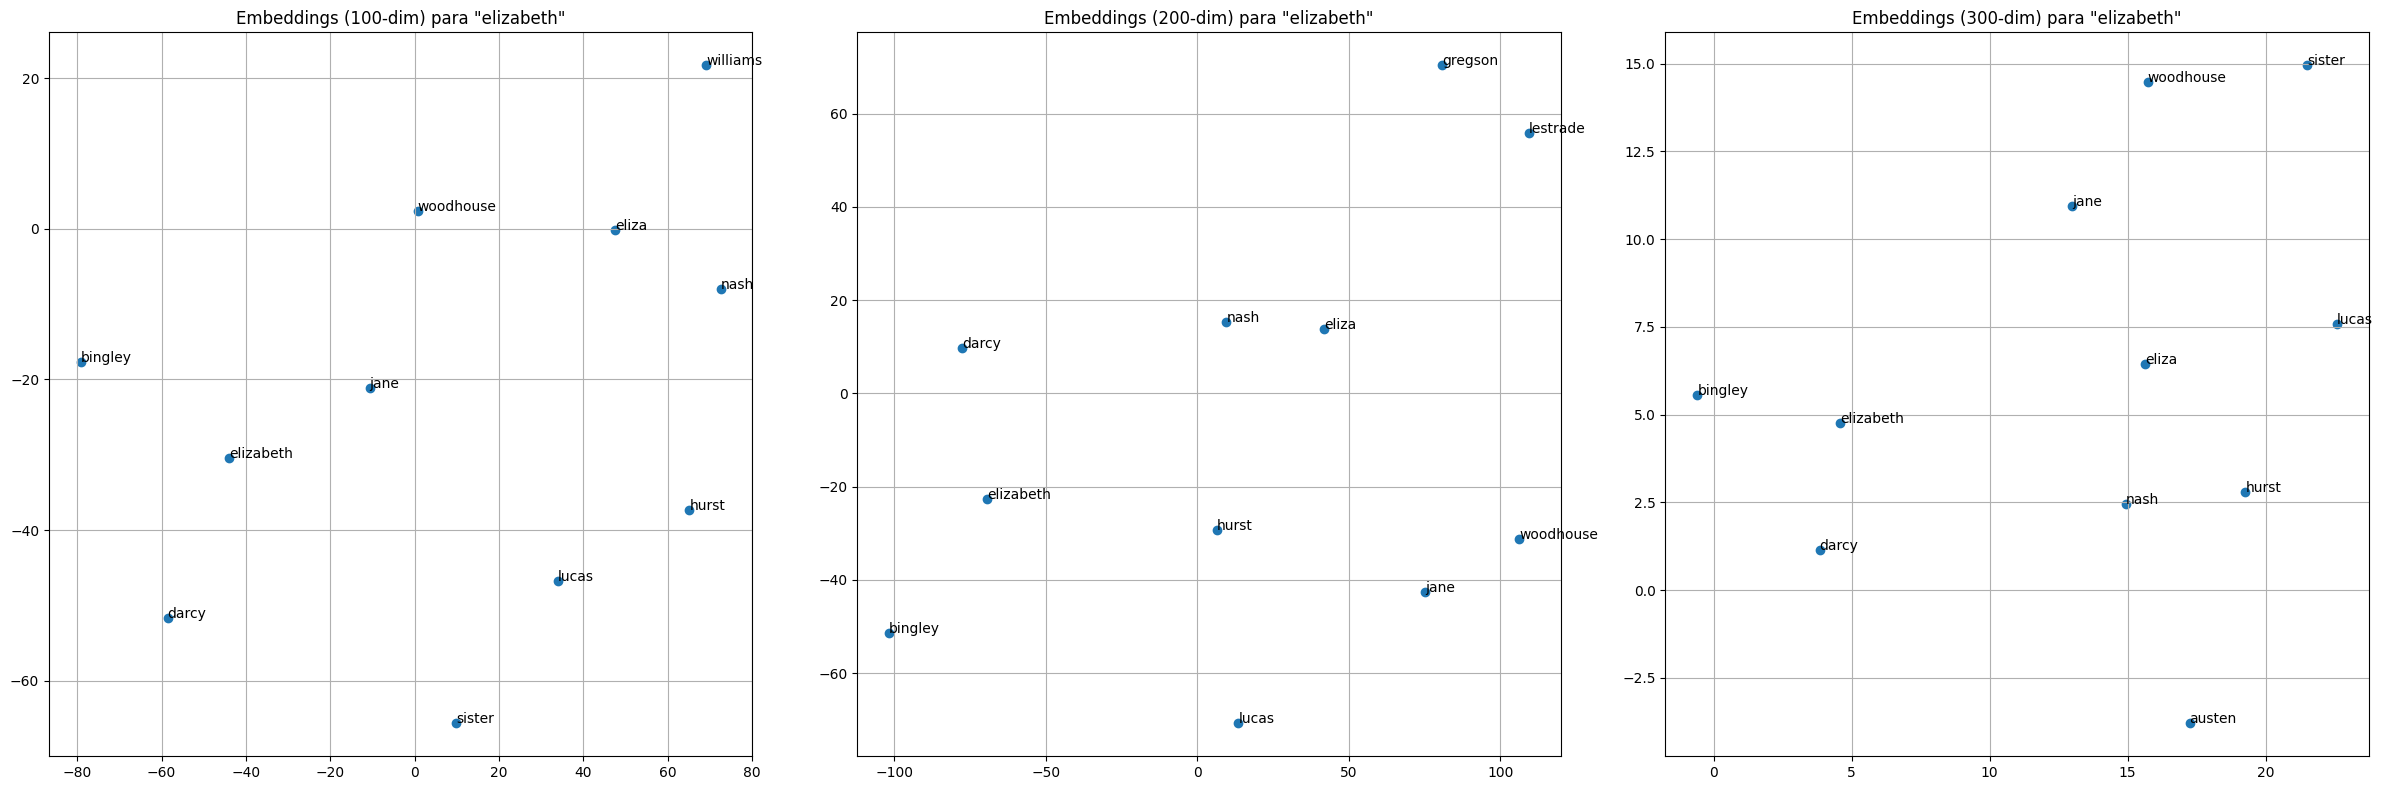
\includegraphics[width=0.9\textwidth]{img/pandp_embeddings.png}
        \caption{Representación 2D de embeddings para "Elizabeth" de "Orgullo y Prejuicio" (100-dim, 200-dim \& 300-dim).}
        \label{fig:pandp_embeddings}
    \end{figure}

    \item En \textbf{Sensatez y Sentimiento}, vamos a centrarnos en las dos hermanas Dashwood principales: "Elinor" y "Marianne". En este, podemos ver su relación con palabras como "Marianne", "afraid" y "ill"; así como con "Elinor", "wished" y "ball", respectivamente.

    \begin{figure}[H]
        \centering
        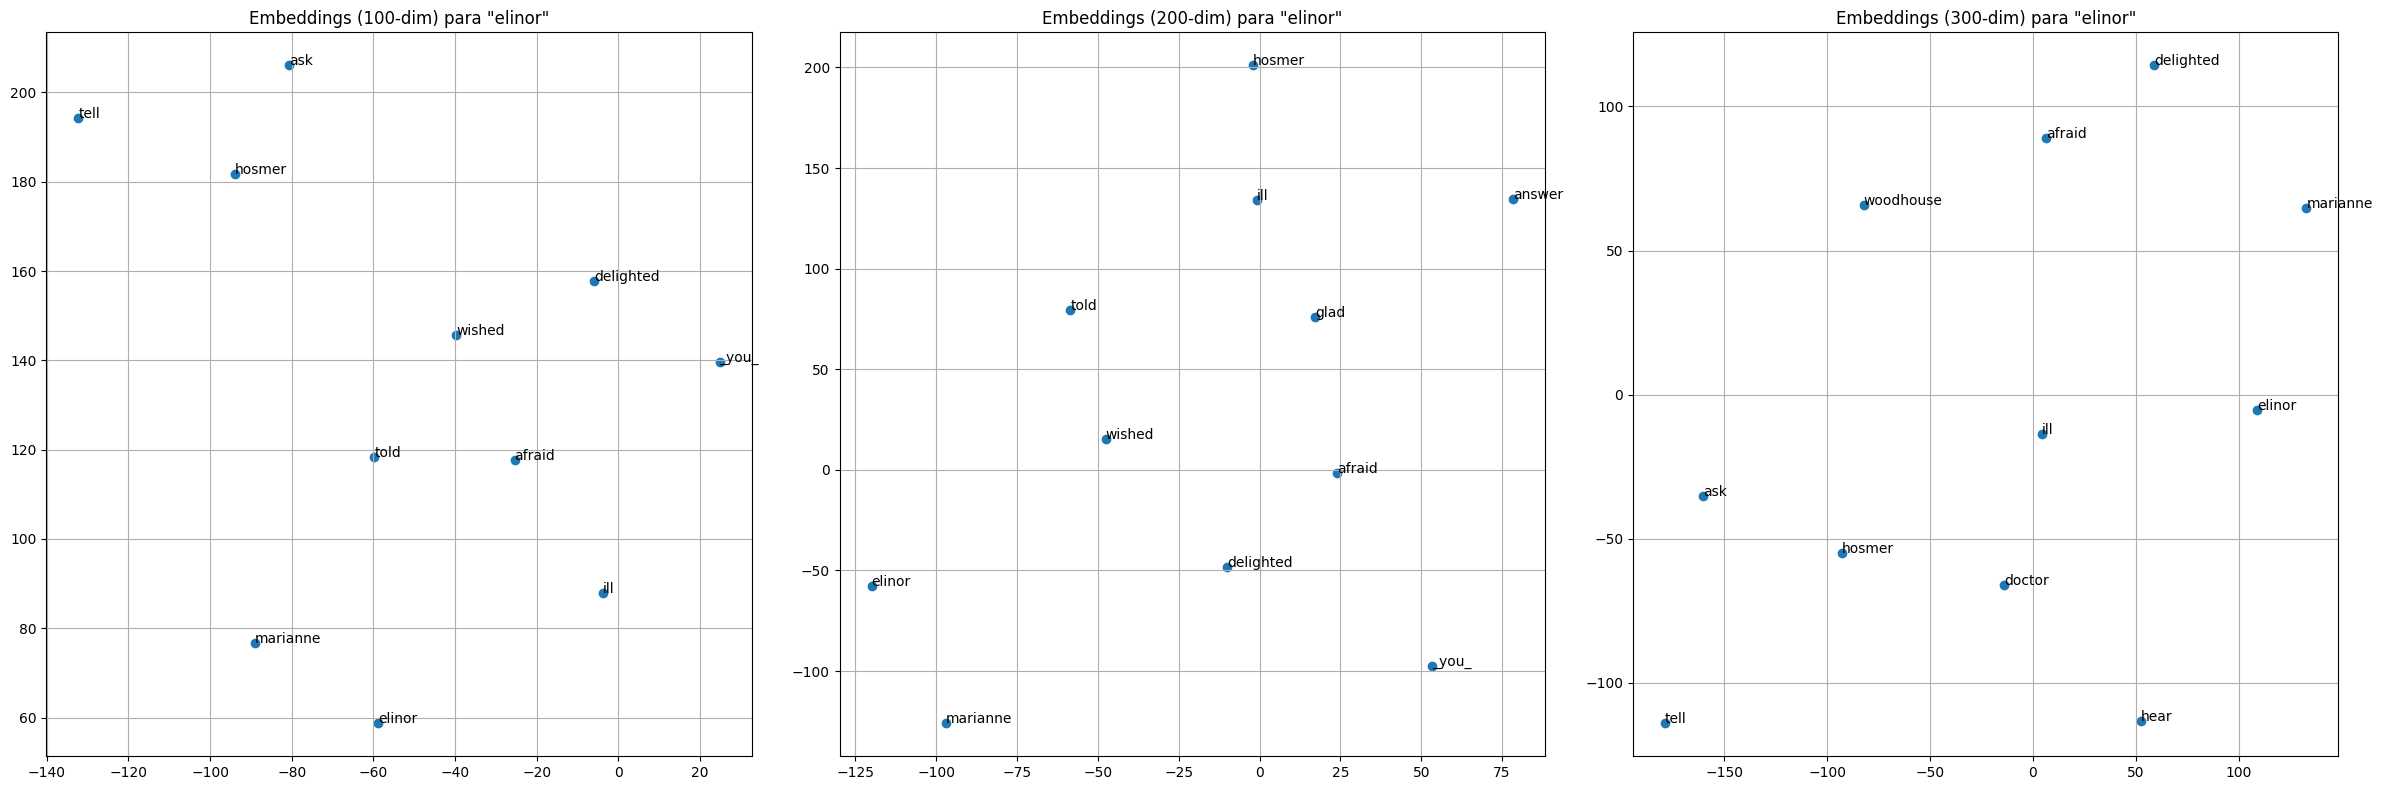
\includegraphics[width=0.9\textwidth]{img/sands_embeddings_elinor.png}
        \caption{Representación 2D de embeddings para "Elinor" de "Sensatez y Sentimiento" (100-dim, 200-dim \& 300-dim).}
        \label{fig:sands_embeddings_elinor}
    \end{figure}

    \begin{figure}[H]
        \centering
        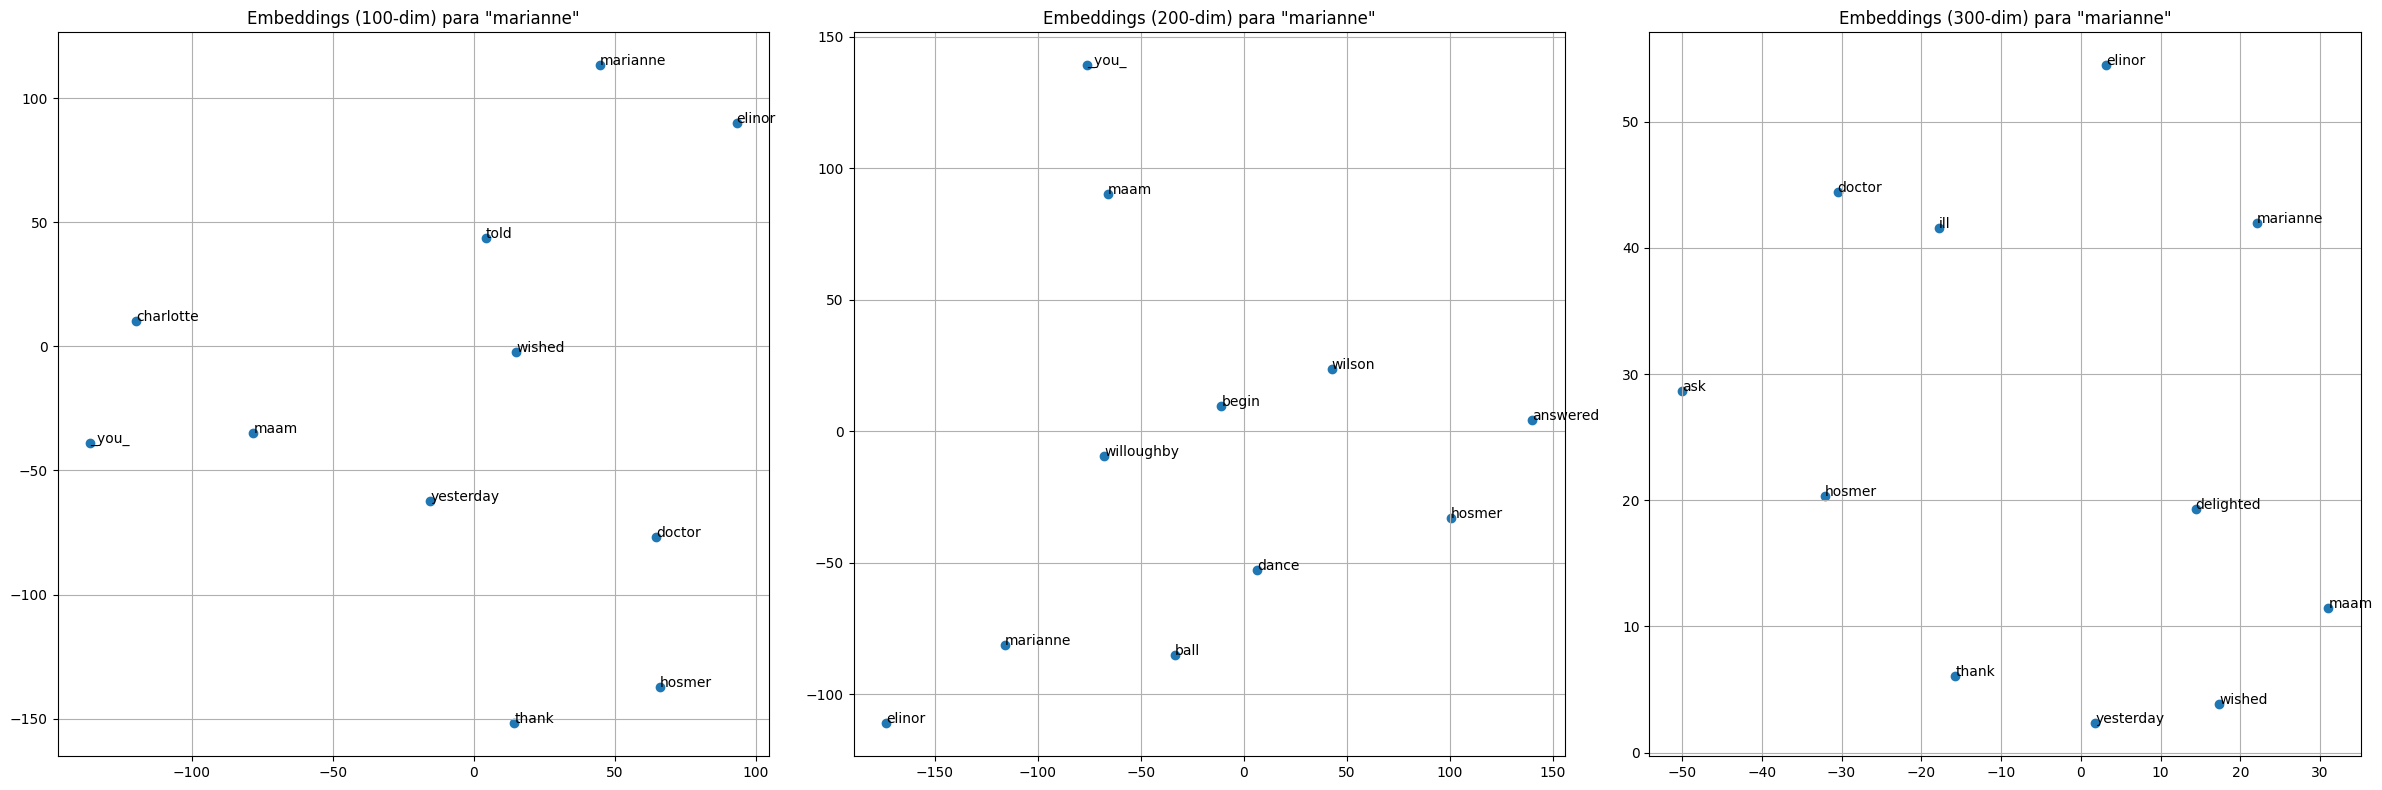
\includegraphics[width=0.9\textwidth]{img/sands_embeddings_marianne.png}
        \caption{Representación 2D de embeddings para "Marianne" de "Sensatez y Sentimiento" (100-dim, 200-dim \& 300-dim).}
        \label{fig:sands_embeddings_marianne}
    \end{figure}

    \item En \textbf{La Caída de la Casa Usher}, podemos visualizar el nombre y apellido del amigo de la infancia del protagonista (dado que este no tiene nombre), Roderick Usher. Sobre este, podemos ver cercanía con palabras como "glorious", "luxury", "scholar", "river", "darkness", "wheel".

    \begin{figure}[H]
        \centering
        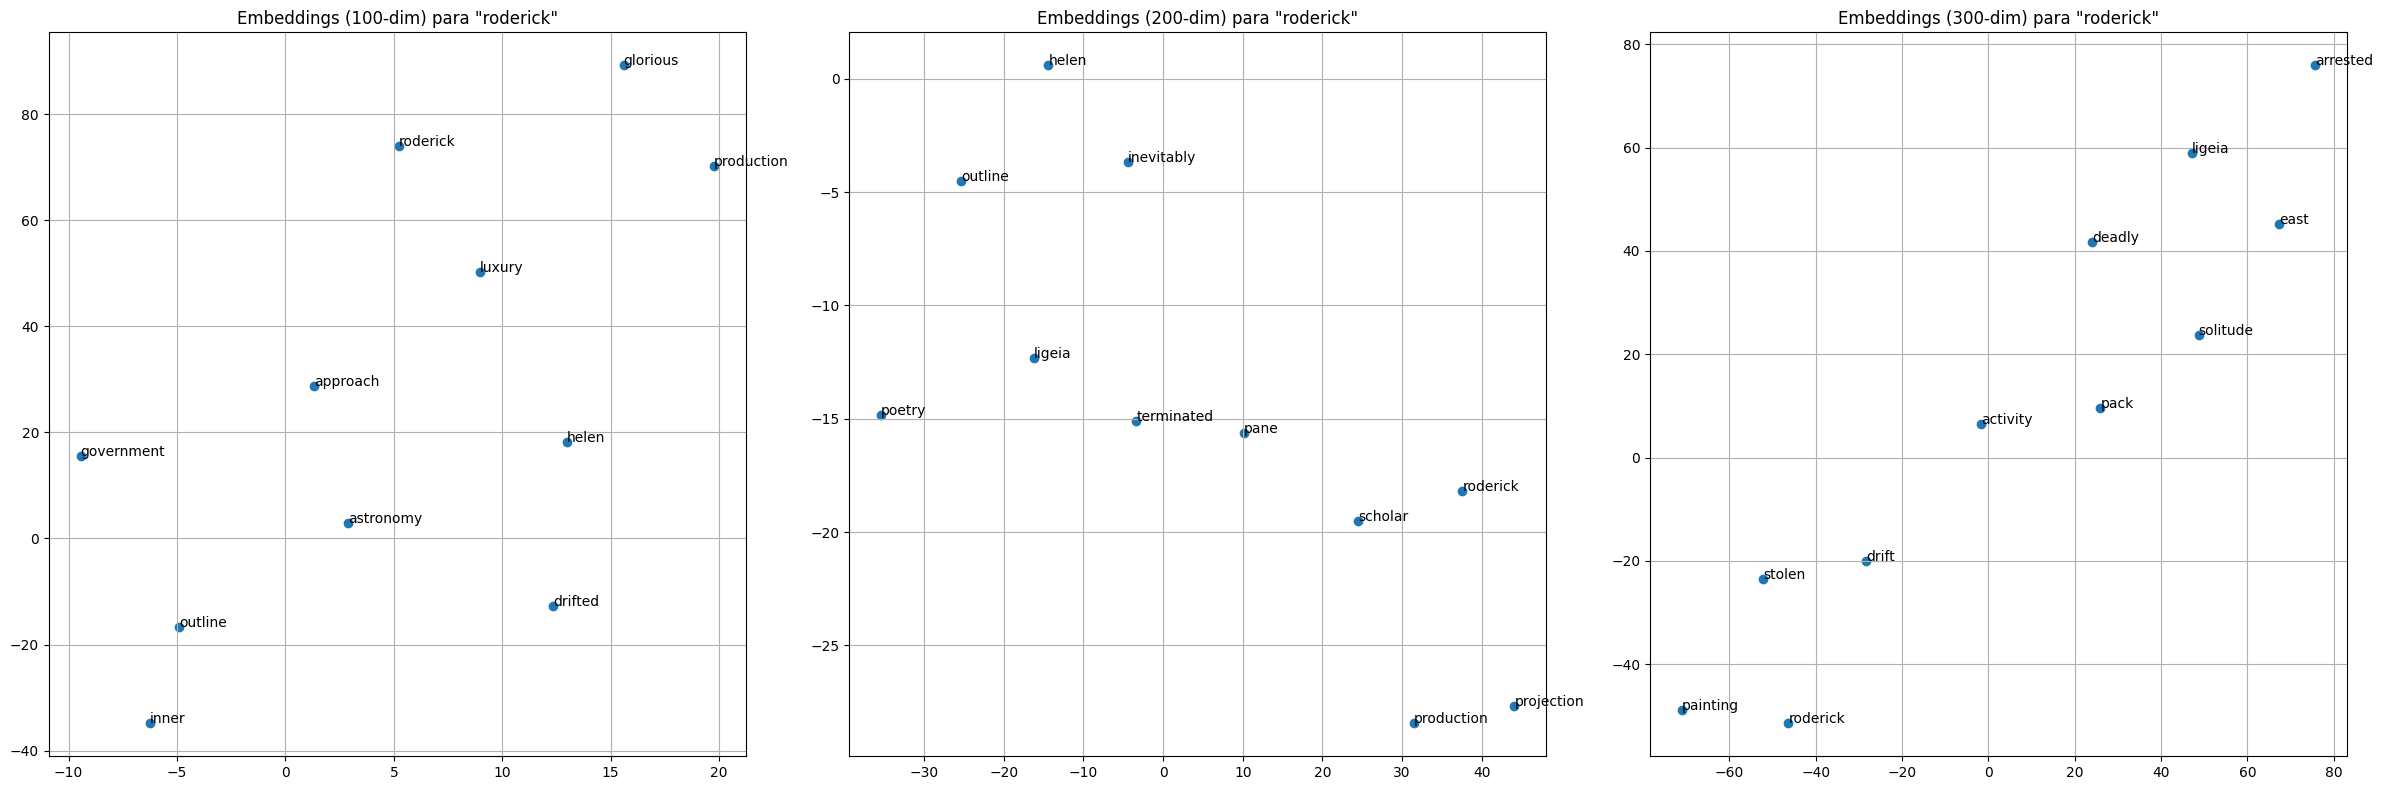
\includegraphics[width=0.9\textwidth]{img/fohu_roderick.png}
        \caption{Representación 2D de embeddings para "Roderick" de "La Caída de la Casa Usher" (100-dim, 200-dim \& 300-dim).}
        \label{fig:fohu_roderick}
    \end{figure}

    \begin{figure}[H]
        \centering
        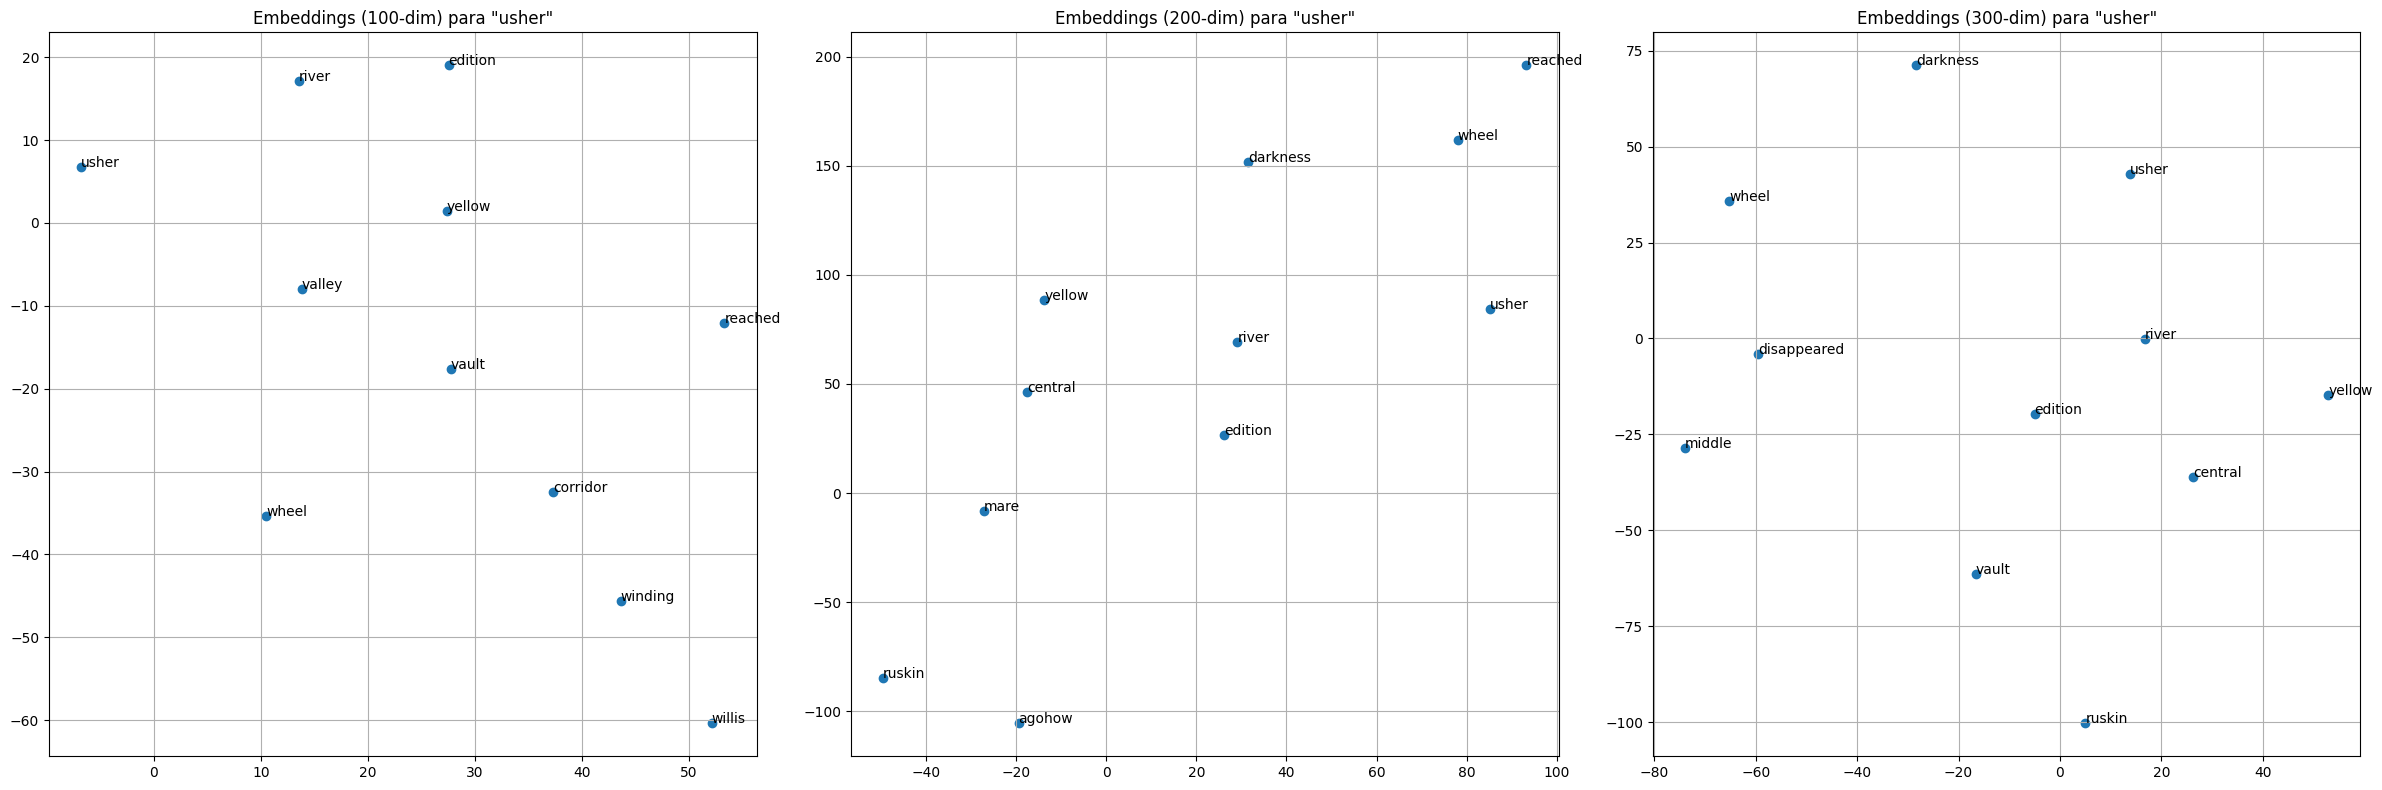
\includegraphics[width=0.9\textwidth]{img/fohu_usher.png}
        \caption{Representación 2D de embeddings para "Usher" de "La Caída de la Casa Usher" (100-dim, 200-dim \& 300-dim).}
        \label{fig:fohu_usher}
    \end{figure}
    
    \item En las obras de Arthur Conan Doyle, visualizamos "Sherlock" y "Watson", mostrando sus conexiones con palabras que frecuentemente coexisten en el contexto del trabajo detectivesco.

    \begin{figure}[H]
        \centering
        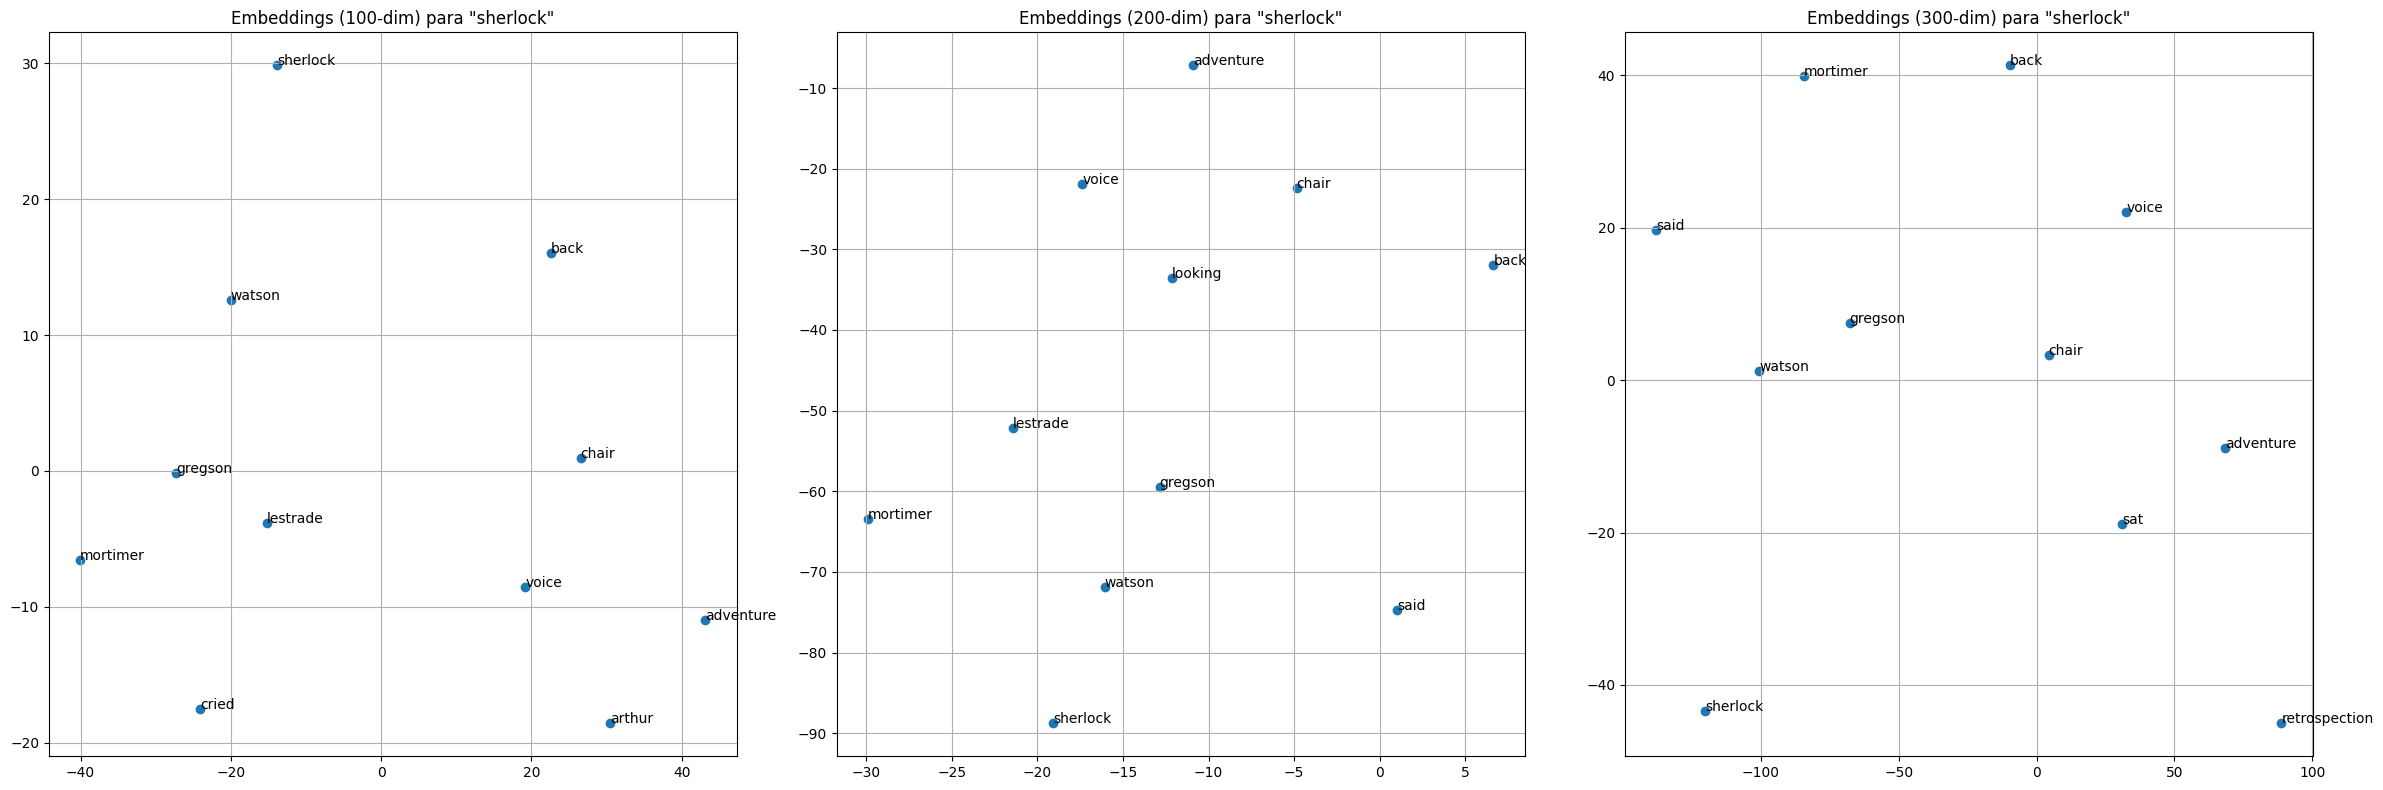
\includegraphics[width=0.9\textwidth]{img/acd_sherlock.png}
        \caption{Representación 2D de embeddings para "Sherlock" en obras de Arthur Conan Doyle (100-dim, 200-dim \& 300-dim).}
        \label{fig:acd_sherlock}
    \end{figure}

    \begin{figure}[H]
        \centering
        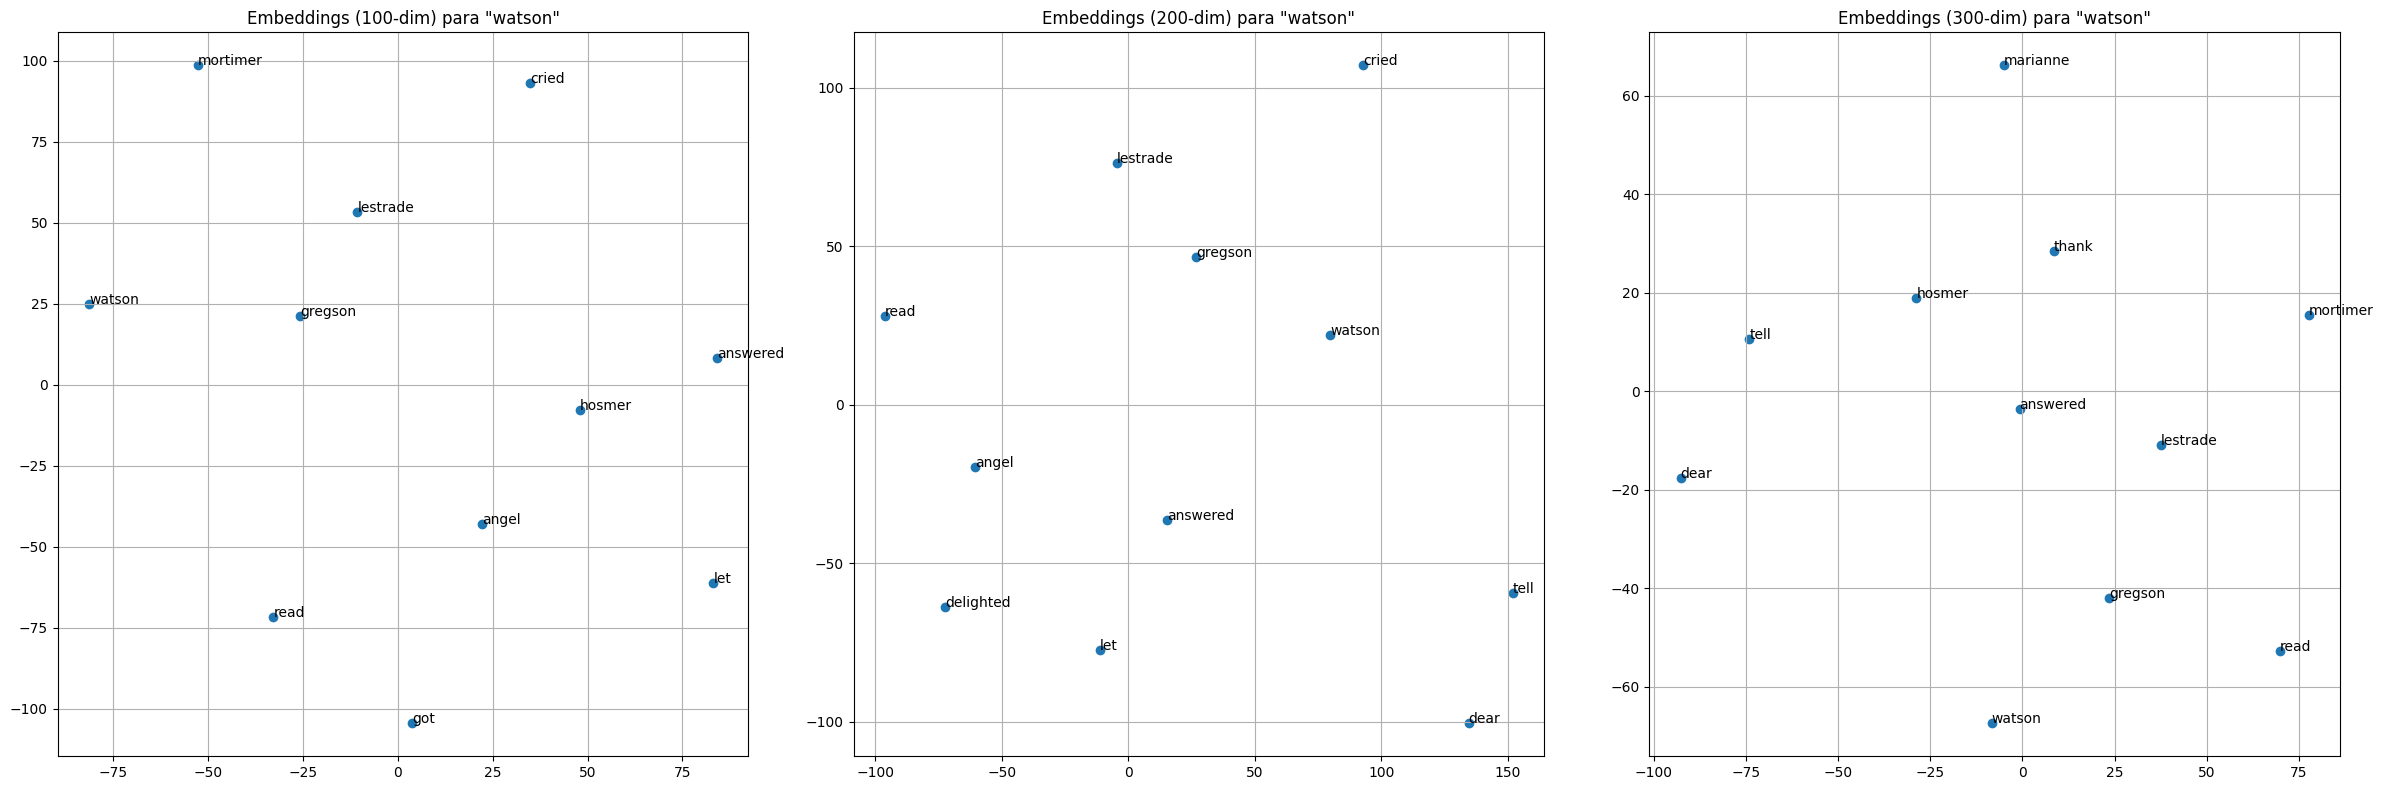
\includegraphics[width=0.9\textwidth]{img/acd_watson.png}
        \caption{Representación 2D de embeddings para "Watson" en obras de Arthur Conan Doyle (100-dim, 200-dim \& 300-dim).}
        \label{fig:acd_watson}
    \end{figure}
    
\end{itemize}

Los resultados de la visualización mostraron claramente que los personajes o conceptos similares tienden a agruparse, validando que el modelo Word2Vec capturó correctamente la estructura semántica de los textos.

\subsection{Extracción de Palabras Clave con TF-IDF}

En aquellos casos donde un libro no tenía un personaje principal claro (como algunas obras de Edgar Allan Poe), aplicamos TF-IDF para identificar términos clave relevantes al texto. Combinando TF-IDF con Word2Vec, pudimos examinar cómo estas palabras importantes se relacionan con otras palabras del corpus. Por ejemplo, en \textbf{The Works of Edgar Allan Poe}, identificamos palabras clave como "time", "body" y "balloon", las cuales se graficaron para mostrar sus relaciones con palabras semánticamente similares en el espacio de Word2Vec.


\begin{figure}[H]
    \centering
    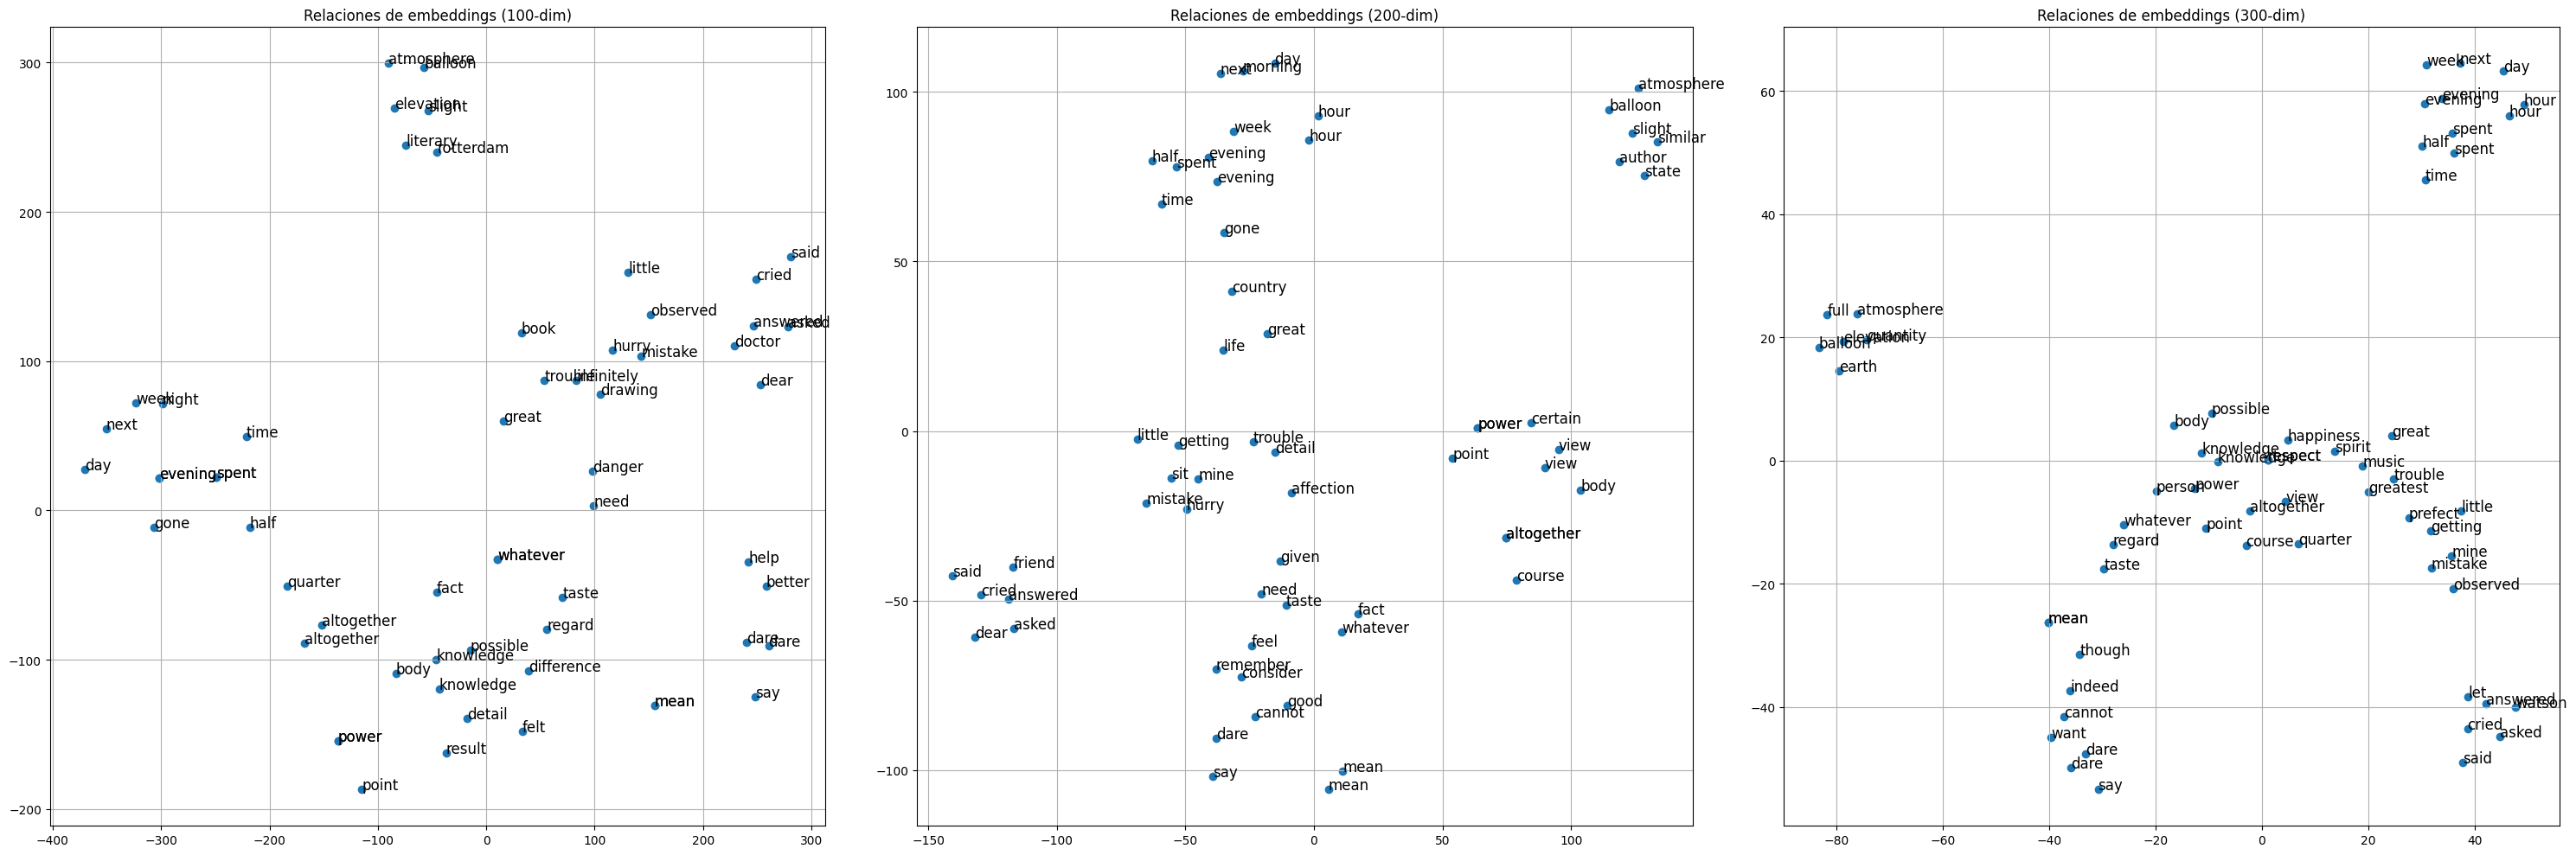
\includegraphics[width=0.9\textwidth]{img/eap_tfidf_vol1.png}
    \caption{Representación 2D de embeddings para palabras clave: "time", "say", "great", "body", "day", "little", "said", "balloon", "mean", "point" en The Works of Edgar Allan Poe Vol. 1 (100-dim, 200-dim \& 300-dim).}
    \label{fig:eap_tfidf_vol1}
\end{figure}

\begin{figure}[H]
    \centering
    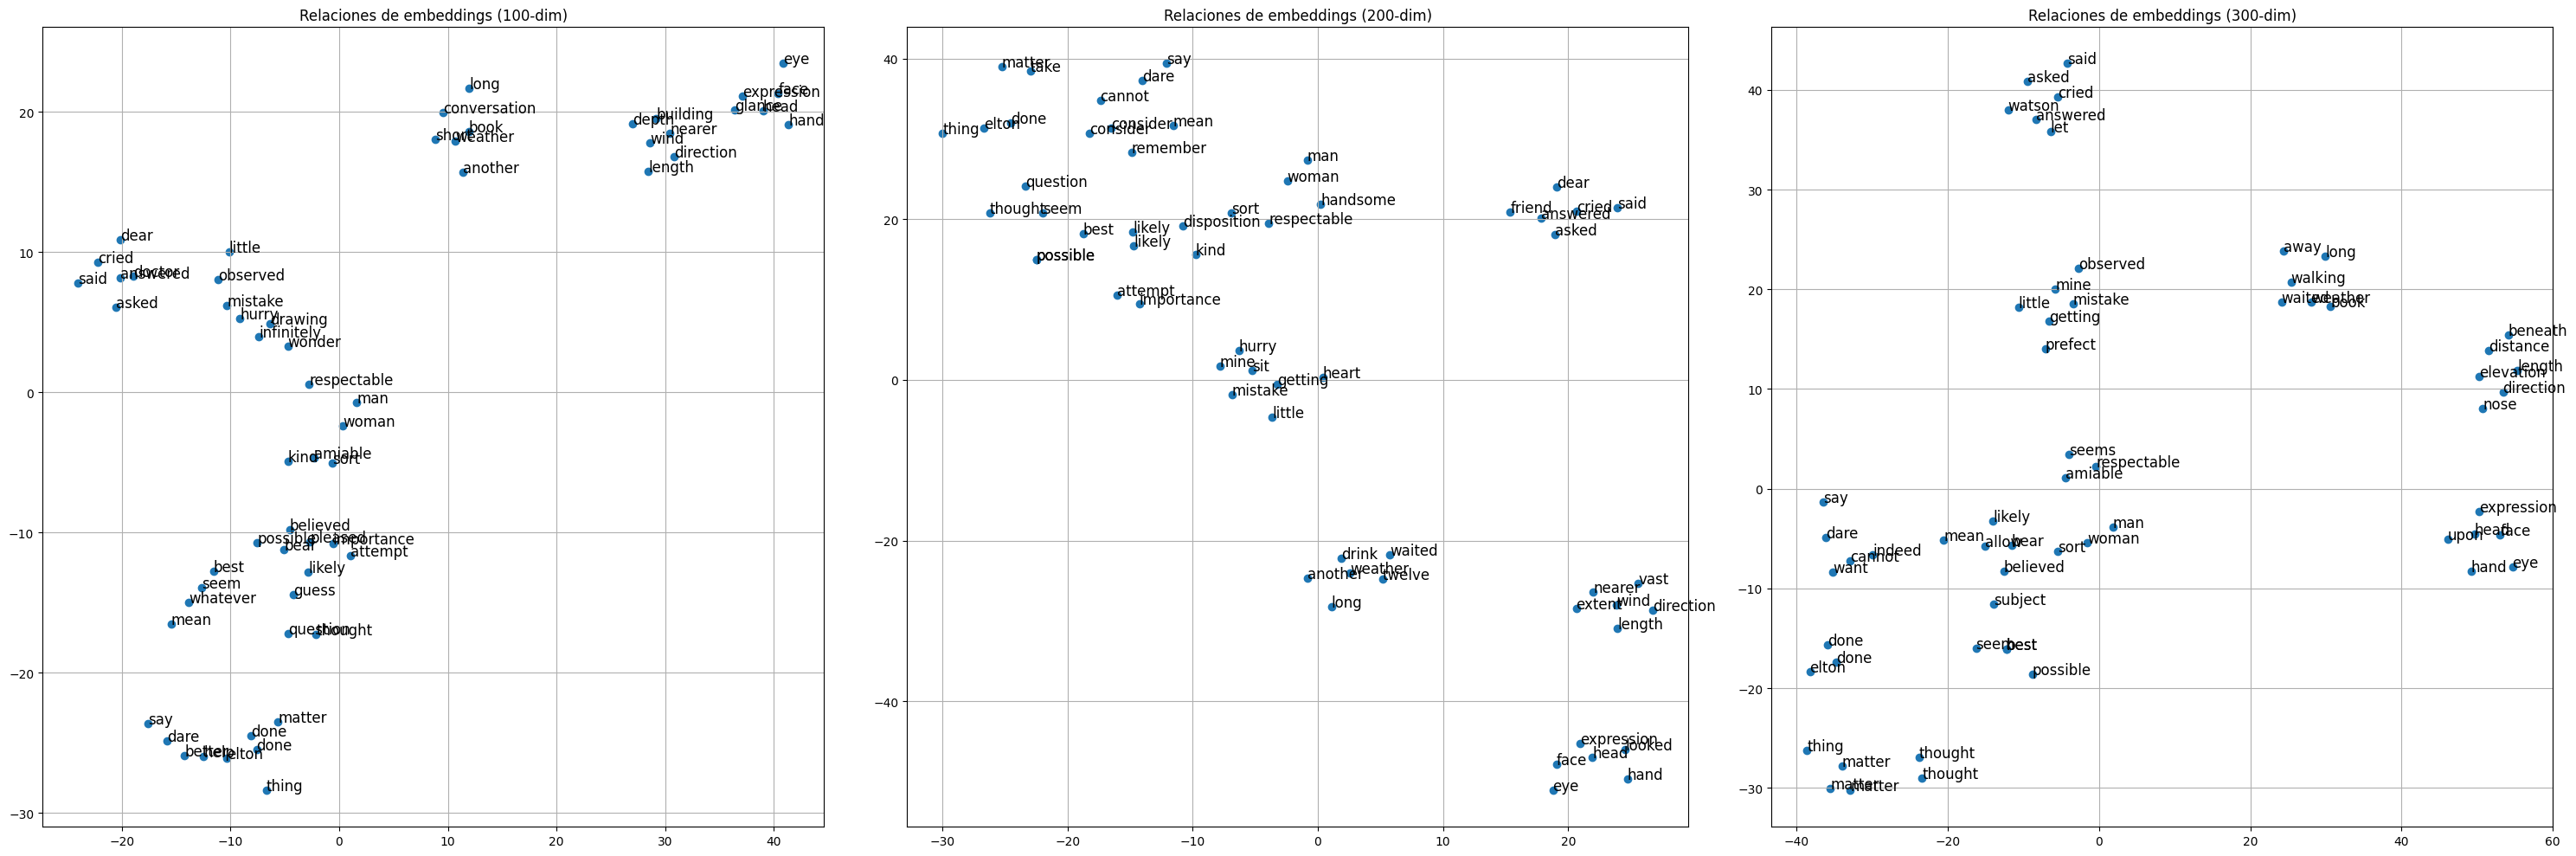
\includegraphics[width=0.9\textwidth]{img/eap_tfidf_vol2.png}
    \caption{Representación 2D de embeddings para palabras clave: "said", "eye", "long", "man", "thing", "thought", "say", "length", "matter", "little" en The Works of Edgar Allan Poe Vol. 2 (100-dim, 200-dim \& 300-dim).}
    \label{fig:eap_tfidf_vol2}
\end{figure}

\subsection{Resumen de Resultados}

El análisis confirmó que Word2Vec capturó eficazmente las relaciones semánticas entre las palabras, con grupos distintivos emergiendo para cada personaje o tema principal en los libros. La combinación de los embeddings de Word2Vec con la visualización t-SNE proporcionó una comprensión intuitiva de cómo se utilizan las palabras en contextos similares a lo largo de diferentes obras literarias.

Al extender el análisis para incluir TF-IDF en textos menos centrados en personajes, pudimos descubrir relaciones semánticas ocultas que no habrían sido tan obvias solo con Word2Vec. Este enfoque dual nos permitió equilibrar el análisis tanto centrado en personajes como en el contenido a lo largo de un corpus diverso.


\section{Modelos de Embeddings}
Se utilizaron dos tipos de embeddings para representar las palabras: Word2Vec y GloVe. Para Word2Vec, se entrenó un modelo en el corpus de libros, y para GloVe, se utilizaron embeddings preentrenados de Wikipedia y Gigaword. Los tamaños de embeddings probados fueron 100, 200 y 300 dimensiones.


\subsection{Arquitecturas de Redes Neuronales}
En esta sección se describen las arquitecturas de las redes neuronales utilizadas para la clasificación y el impacto de las diferentes dimensionalidades de embeddings (Word2Vec y GloVe) en el rendimiento del modelo. Además, se comparan los resultados obtenidos con embeddings preentrenados y embeddings personalizados.

Definimos tres arquitecturas de redes neuronales densas en Keras, con un número creciente de capas y neuronas en cada arquitectura. A continuación, se detallan las configuraciones:

\begin{itemize}
    \item \textbf{Arquitectura 1:} Una red simple con una única capa densa de 128 neuronas. Utiliza activación ReLU y Dropout para evitar el sobreajuste.
    \begin{itemize}
        \item Input: Embedding de $n$ dimensiones, según la configuración del embedding.
        \item Capa Densa: 128 neuronas, activación ReLU.
        \item Dropout: Tasa de 0.3.
        \item Capa de salida: 3 neuronas con activación softmax (para la clasificación de los tres autores).
    \end{itemize}
    
    \item \textbf{Arquitectura 2:} Esta arquitectura añade una capa intermedia adicional.
    \begin{itemize}
        \item Input: Embedding de $n$ dimensiones.
        \item Capa Densa 1: 256 neuronas, activación ReLU.
        \item Dropout: Tasa de 0.3.
        \item Capa Densa 2: 128 neuronas, activación ReLU.
        \item Dropout: Tasa de 0.3.
        \item Capa de salida: 3 neuronas con activación softmax.
    \end{itemize}
    
    \item \textbf{Arquitectura 3:} Un modelo más profundo con tres capas densas.
    \begin{itemize}
        \item Input: Embedding de $n$ dimensiones.
        \item Capa Densa 1: 512 neuronas, activación ReLU.
        \item Dropout: Tasa de 0.3.
        \item Capa Densa 2: 256 neuronas, activación ReLU.
        \item Dropout: Tasa de 0.3.
        \item Capa Densa 3: 128 neuronas, activación ReLU.
        \item Dropout: Tasa de 0.3.
        \item Capa de salida: 3 neuronas con activación softmax.
    \end{itemize}
\end{itemize}

Estas arquitecturas permiten observar el impacto del número de neuronas y capas en la precisión del modelo, así como la relación entre complejidad de la red y el tamaño de los embeddings.

\subsection{Entrenamiento del Clasificador}

Los modelos fueron entrenados utilizando la función de pérdida \texttt{categorical\_crossentropy} y el optimizador \texttt{Adam}, con una tasa de aprendizaje inicial de $1e^{-3}$. Implementamos \texttt{EarlyStopping} para detener el entrenamiento si no había mejoras en la métrica de pérdida en el conjunto de validación durante 5 épocas consecutivas. También usamos \texttt{ModelCheckpoint} para guardar los pesos del mejor modelo.

Cada arquitectura se entrenó durante un máximo de 50 épocas, con un \textit{batch size} de 32. Dividimos el dataset en 70\% para entrenamiento, 15\% para validación, y 15\% para pruebas.

\subsection{Evaluación del Rendimiento}

Las métricas utilizadas para la evaluación de los modelos fueron exactitud, precisión y recall. A continuación, se resumen los resultados más destacados:

\subsubsection{Resultados con Word2Vec Embeddings}

En la tabla \ref{tab:word2vec}, observamos los resultados obtenidos al usar los embeddings personalizados de Word2Vec con diferentes dimensiones de embedding.

\begin{table}[H]
    \centering
    \caption{Resultados con Word2Vec Embeddings (Precisión, Exactitud y Recall)}
    \label{tab:word2vec}
    \begin{tabular}{|c|c|c|c|c|}
    \hline
    \textbf{Arquitectura} & \textbf{Tamaño Embedding} & \textbf{Exactitud} & \textbf{Precisión} & \textbf{Recall} \\
    \hline
    Arquitectura 1 & 100 & 0.747 & 0.773 & 0.747 \\
    Arquitectura 2 & 100 & 0.769 & 0.778 & 0.769 \\
    Arquitectura 3 & 100 & 0.762 & 0.765 & 0.762 \\
    Arquitectura 1 & 200 & 0.747 & 0.749 & 0.747 \\
    Arquitectura 2 & 200 & 0.769 & 0.774 & 0.769 \\
    Arquitectura 3 & 200 & 0.780 & 0.799 & 0.780 \\
    Arquitectura 1 & 300 & 0.755 & 0.752 & 0.755 \\
    Arquitectura 2 & 300 & 0.773 & 0.788 & 0.772 \\
    Arquitectura 3 & 300 & 0.729 & 0.781 & 0.729 \\
    \hline
    \end{tabular}
\end{table}

\begin{figure}[H]
    \centering
    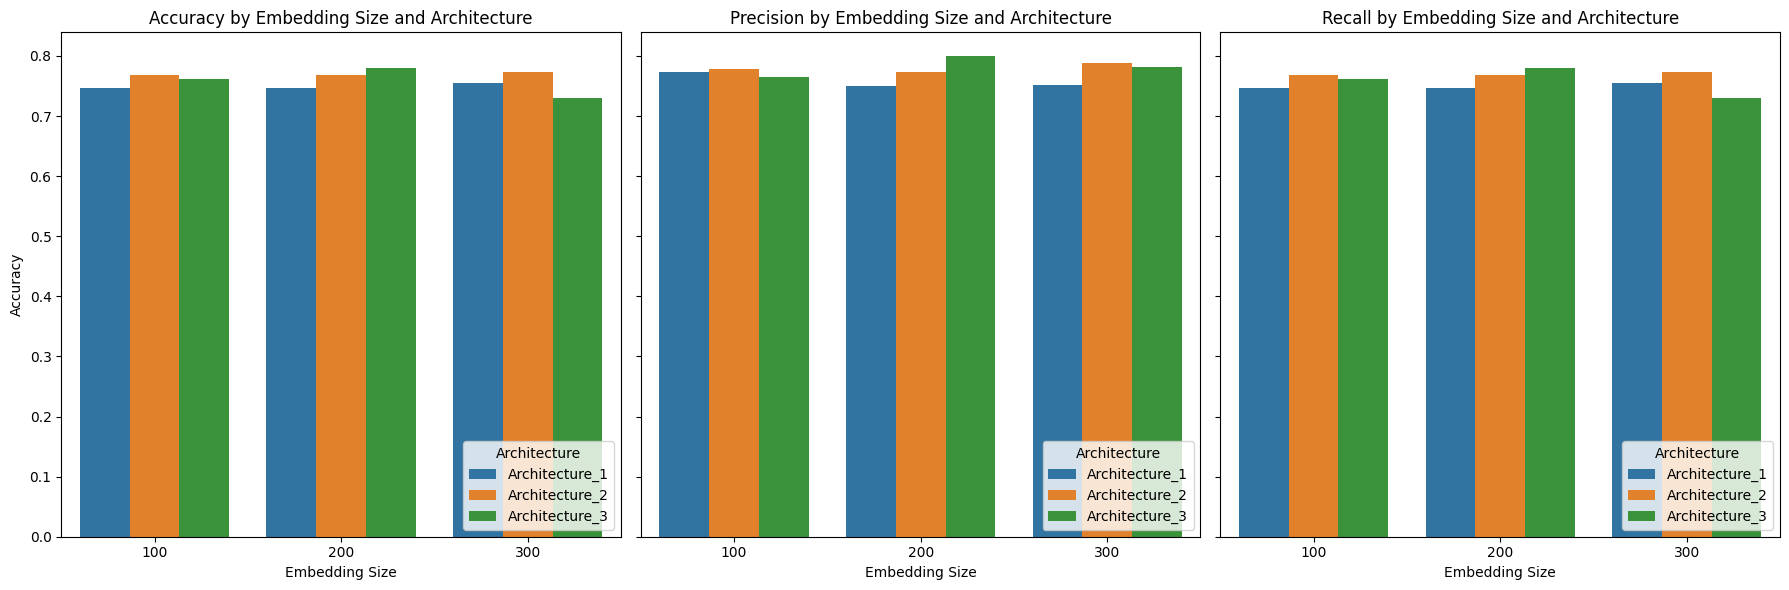
\includegraphics[width=0.8\textwidth]{img/embeddings_no_glove.png}
    \caption{Gráficas de métricas de resultados con Word2Vex Embeddings.}
    \label{fig:embeddings_no_glove}
\end{figure}

Se observa que la arquitectura más compleja (Arquitectura 3) con embeddings de tamaño 200 presentó el mejor rendimiento, alcanzando una precisión del 79.9\%.

\subsubsection{Resultados con Embeddings Preentrenados de GloVe}

La tabla \ref{tab:glove} muestra los resultados al usar embeddings preentrenados de GloVe con diferentes dimensiones de embedding.

\begin{table}[H]
    \centering
    \caption{Resultados con GloVe Embeddings (Precisión, Exactitud y Recall)}
    \label{tab:glove}
    \begin{tabular}{|c|c|c|c|c|}
    \hline
    \textbf{Arquitectura} & \textbf{Tamaño Embedding} & \textbf{Exactitud} & \textbf{Precisión} & \textbf{Recall} \\
    \hline
    Arquitectura 1 & 100 & 0.722 & 0.717 & 0.722 \\
    Arquitectura 2 & 100 & 0.693 & 0.684 & 0.693 \\
    Arquitectura 3 & 100 & 0.693 & 0.687 & 0.693 \\
    Arquitectura 1 & 200 & 0.708 & 0.703 & 0.708 \\
    Arquitectura 2 & 200 & 0.708 & 0.700 & 0.798 \\
    Arquitectura 3 & 200 & 0.682 & 0.676 & 0.682 \\
    Arquitectura 1 & 300 & 0.733 & 0.727 & 0.733 \\
    Arquitectura 2 & 300 & 0.762 & 0.759 & 0.762 \\
    Arquitectura 3 & 300 & 0.704 & 0.713 & 0.704 \\
    \hline
    \end{tabular}
\end{table}

\begin{figure}[H]
    \centering
    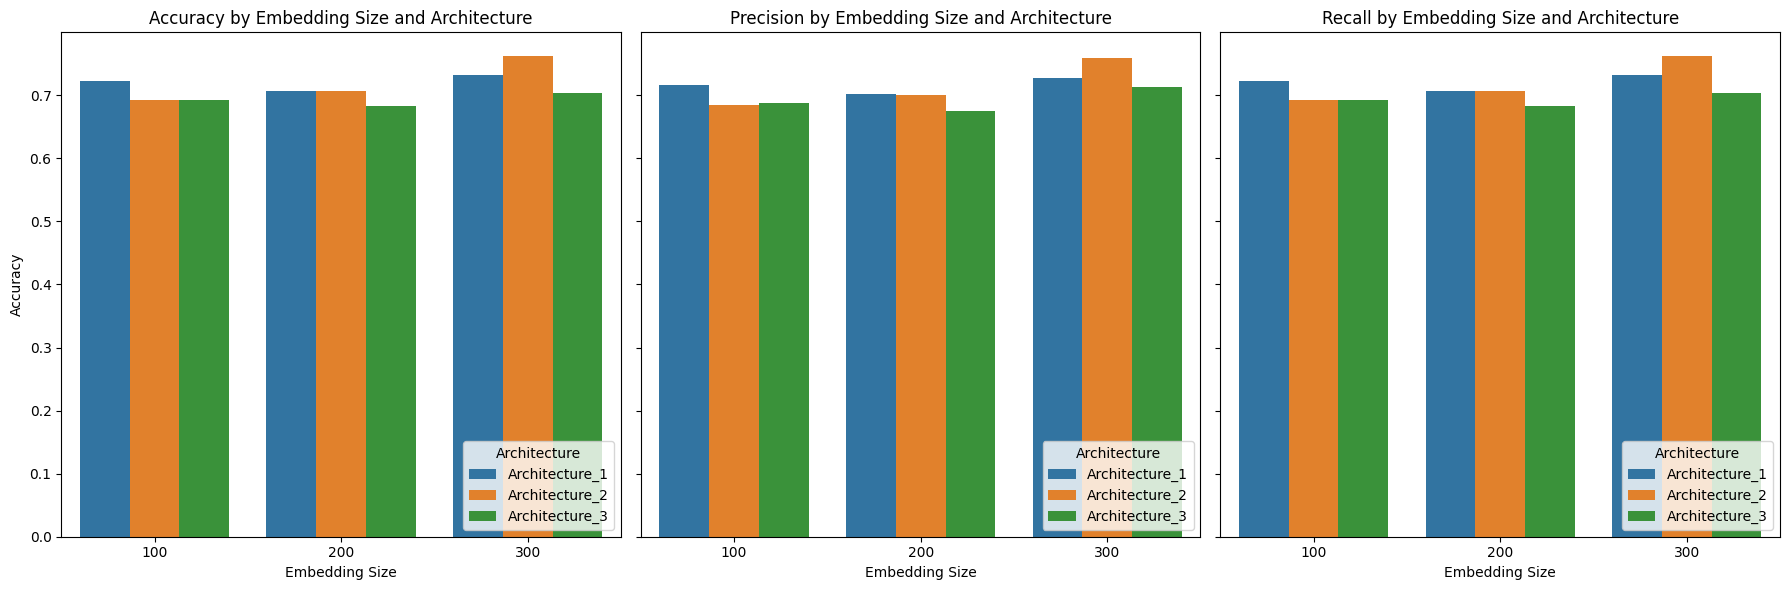
\includegraphics[width=0.8\textwidth]{img/embeddings_glove.png}
    \caption{Gráficas de métricas de resultados con GloVe Embeddings.}
    \label{fig:embeddings_glove}
\end{figure}

Al comparar los resultados de Word2Vec y GloVe, encontramos que Word2Vec personalizado tiende a ofrecer mejores resultados, especialmente cuando se utilizan embeddings más pequeños (100 y 200 dimensiones).

\subsection{Análisis Comparativo}

\subsubsection{Embeddings Personalizados vs. Preentrenados}

Los resultados muestran que los embeddings personalizados de Word2Vec entrenados en el corpus específico de libros presentan un mejor rendimiento que los embeddings preentrenados de GloVe, especialmente en el caso de los embeddings de menor dimensionalidad (100 y 200). Esto sugiere que los embeddings personalizados capturan mejor las características semánticas relevantes de los libros de los tres autores seleccionados.

Sin embargo, los embeddings de GloVe preentrenados muestran una mejora en términos de generalización cuando se utilizan embeddings más grandes (300 dimensiones), posiblemente porque incluyen una mayor variedad de contexto global que podría no estar presente en los embeddings personalizados.

\subsubsection{Impacto de la Dimensionalidad de Embeddings}

La dimensionalidad del embedding influye directamente en el rendimiento del modelo. Los embeddings de menor tamaño (100) tienden a ser más eficientes para tareas más simples, mientras que los embeddings de mayor tamaño (200 o 300) proporcionan un mejor rendimiento en redes neuronales más complejas (Arquitectura 3).

La elección de la dimensionalidad debe equilibrar la precisión del modelo con los costos computacionales, ya que los embeddings más grandes requieren más tiempo de entrenamiento y recursos, pero no siempre garantizan una mejora significativa en los resultados.

\section{Conclusiones}

\begin{itemize}
    \item Las arquitecturas más complejas con embeddings de mayor tamaño tienden a ofrecer un mejor rendimiento en términos de precisión, especialmente cuando se utilizan embeddings de Word2Vec entrenados en el corpus específico.
    \item Los embeddings preentrenados como GloVe ofrecen un rendimiento competitivo, pero los resultados indican que los embeddings personalizados son más efectivos para capturar las relaciones semánticas dentro de un dominio de corpus especializado.
    \item La dimensionalidad del embedding tiene un impacto significativo en el rendimiento, y el mejor balance entre precisión y costos computacionales se logró con embeddings de tamaño 200, combinado con la arquitectura más compleja (Arquitectura 3).
\end{itemize}

Finalmente, podemos observar que las arquitecturas más complejas con embeddings de mayor tamaño tienden a mejorar ligeramente las métricas de evaluación. El mejor rendimiento general se alcanzó con la Arquitectura 3 y embeddings de tamaño 300, obteniendo una precisión del 79.9\% y un recall del 78\% utilizando Word2Vec. Sin embargo, el uso de GloVe también mostró resultados competitivos.
\end{document}